\chapter{Introdução}

A criptografia quântica é um campo em rápido desenvolvimento que usa os princípios da mecânica quântica para transmitir e proteger informações. A história da criptografia quântica remonta à década de 1980, quando os pesquisadores começaram a explorar o potencial de usar sistemas quânticos para codificar e transmitir informações de maneira segura contra espionagem e outros ataques.

Os princípios da criptografia quântica são baseados nos princípios fundamentais da mecânica quântica, incluindo o princípio da incerteza, entrelaçamento e superposição. Esses princípios permitem a criação de chaves criptográficas seguras que podem ser usadas para codificar e descodificar informações transmitidas por um canal quântico.

Um dos principais protocolos na criptografia quântica é o protocolo Quantum Key Distribution (QKD), que permite a troca segura de chaves criptográficas em um canal quântico. Este protocolo é baseado nos princípios da mecânica quântica e é projetado para ser seguro contra uma variedade de ataques, incluindo aqueles que exploram as leis da física clássica.

Apesar das muitas vantagens da criptografia quântica, também existem limitações que devem ser consideradas. Por exemplo, a transmissão de informações por um canal quântico está sujeita a perdas e ruídos, o que pode limitar a eficácia dos protocolos QKD. Além disso, também existem possíveis vulnerabilidades de segurança que devem ser abordadas, como ataques que exploram canais laterais ou outras deficiências no sistema quântico.

Para lidar com essas limitações, os pesquisadores propuseram várias soluções potenciais, incluindo o uso de técnicas avançadas de correção de erros e novos protocolos que vão além do QKD tradicional. Neste artigo, exploraremos a história e os princípios da criptografia quântica, suas limitações e possíveis soluções, os principais protocolos usados na criptografia quântica e as perspectivas futuras desse campo empolgante.

\begin{figure}[!hbt]
  \centering
  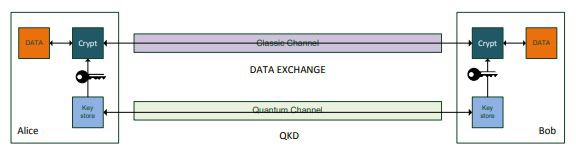
\includegraphics[width=\textwidth]{images/intro.jpg}
  \caption{Figura ilustrativa da criptografia quântica.}
  \label{fig:intro}
\end{figure}
\FloatBarrier

\newpage
